\documentclass[10pt,reqno]{article}
\usepackage{import}

\usepackage{tikz}
\usetikzlibrary{shapes,arrows,positioning,decorations,decorations.pathreplacing,quotes,angles}

% ------- general -------
\usepackage{amsmath} % symbols
\usepackage{amssymb} % symbols, \mathfrak
\usepackage{amsthm} % theorems, proofs, etc
%\usepackage{dutchcal} % replaces \mathcal

\usepackage{eucal}

\usepackage{dsfont} % symbols
\usepackage{mathtools}
\usepackage{amsfonts}
% \usepackage{wasysym} % symbols
\usepackage{gensymb} % degree symbol \degree


\usepackage{graphicx}
\usepackage{caption}
\usepackage{subcaption}

\usepackage{float}

\usepackage[
a4paper,
left=3.5cm,
right=3.5cm,
top=2cm,
bottom=2cm
]{geometry}
\renewcommand{\qedsymbol}{\ensuremath{\blacksquare}}


\newtheoremstyle{erd-thm}
{}                % Space above
{}                % Space below
{\slshape}        % Theorem body font % (default is "\upshape")
{}                % Indent amount
{\bfseries}       % Theorem head font % (default is \mdseries)
{.}               % Punctuation after theorem head % default: no punctuation
{0.5em}               % Space after theorem head
{}                % Theorem head spec

\newtheoremstyle{erd-defn}
{}                % Space above
{}                % Space below
{\upshape}        % Theorem body font % (default is "\upshape")
{}                % Indent amount
{\bfseries}       % Theorem head font % (default is \mdseries)
{.}               % Punctuation after theorem head % default: no punctuation
{0.5em}               % Space after theorem head
{}                % Theorem head spec

\newtheoremstyle{erd-rem}
{}                % Space above
{}                % Space below
{\upshape}        % Theorem body font % (default is "\upshape")
{}                % Indent amount
{\slshape}       % Theorem head font % (default is \mdseries)
{.}               % Punctuation after theorem head % default: no punctuation
{0.5em}  % Space after theorem head
{}                % Theorem head spec

%\swapnumbers
\theoremstyle{erd-thm}
\newtheorem{theorem}{Theorem}[section]
\newtheorem{corollary}[theorem]{Corollary}
\newtheorem{lemma}[theorem]{Lemma}
\newtheorem{conjecture}[theorem]{Conjecture}
\newtheorem{proposition}[theorem]{Proposition}
\newtheorem{postulate}[theorem]{Postulate}

\theoremstyle{erd-defn}
\newtheorem{definition}[theorem]{Definition}
\newtheorem{notation}[theorem]{Notation}
\newtheorem{example}[theorem]{Example}
\newtheorem{counterexample}[theorem]{Counterexample}
\newtheorem{exercise}[theorem]{Exercise}
\newtheorem{opgave}{Opgave}

\theoremstyle{erd-rem}
\newtheorem{remark}[theorem]{Remark}
\newtheorem{claim}[theorem]{Claim}
\newtheorem{conclusion}[theorem]{Conclusion}

% ------ unnumbered ------
\theoremstyle{erd-thm}
\newtheorem*{theorem*}{Theorem}
\newtheorem*{corollary*}{Corollary}
\newtheorem*{lemma*}{Lemma}
\newtheorem*{conjecture*}{Conjecture}
\newtheorem*{proposition*}{Proposition}
\newtheorem{postulate*}{Postulate}

\theoremstyle{erd-defn}
\newtheorem*{definition*}{Definition}
\newtheorem*{example*}{Example}
\newtheorem*{counterexample*}{Counterexample}
\newtheorem*{exercise*}{Exercise}

\theoremstyle{erd-rem}
\newtheorem*{remark*}{Remark}
\newtheorem*{claim*}{Claim}
\newtheorem*{conclusion*}{Conclusion}

\newcommand{\field}[1]{\mathbb{#1}}


% ---------------
%   M A C R O S
% ---------------

\newcommand{\defeq}{\overset{\underset{\mathrm{def}}{}}{=}}

\DeclareMathOperator{\id}{id}
\DeclareMathOperator{\Id}{Id}

\newcommand{\isom}{\simeq} % \cong

\DeclareMathOperator{\Hom}{Hom}
\DeclareMathOperator{\Obj}{Obj}
\DeclareMathOperator{\Cone}{Cone}
\DeclareMathOperator{\Cones}{Cones}
\DeclareMathOperator{\Cocone}{Cocone}
\DeclareMathOperator{\colim}{colim}
\DeclareMathOperator{\coeq}{coeq}

\DeclareMathOperator{\Int}{Int}

\DeclareMathOperator{\Ree}{Re}
\DeclareMathOperator{\Imm}{Im}

\DeclareMathOperator{\Alt}{Alt}
\DeclareMathOperator{\adj}{adj}
\DeclareMathOperator{\vspan}{span}

\DeclareMathOperator{\Inn}{Inn}
\DeclareMathOperator{\Aut}{Aut}
\DeclareMathOperator{\End}{End}
\DeclareMathOperator{\Sym}{Sym}
\DeclareMathOperator{\Char}{char}
\DeclareMathOperator{\Cl}{Cl}


\DeclareMathOperator{\supp}{supp}

\DeclareMathOperator{\eq}{eq}
\DeclareMathOperator{\sgn}{sgn}
\DeclareMathOperator{\ggd}{ggd}
\DeclareMathOperator{\kgv}{kgv}
\DeclareMathOperator{\Aff}{Aff}
\DeclareMathOperator{\GL}{GL}
\DeclareMathOperator{\PGL}{PGL}
\DeclareMathOperator{\SL}{SL}
\DeclareMathOperator{\Tr}{Tr}

\DeclareMathOperator{\diam}{diam}

\DeclareMathOperator{\dom}{dom}
\DeclareMathOperator{\cod}{cod}

\DeclareMathOperator{\Exp}{Exp}


\DeclareMathOperator{\Var}{Var}
\DeclareMathOperator{\Cov}{Cov}


\renewcommand{\vec}[1]{\mathbf{#1}}

\newcommand{\dsqrt}[2][2]{
	\sqrt[\leftroot{0}\uproot{2}#1]{}
}



\renewcommand{\P}{\mathds{P}}
\newcommand{\A}{\mathds{A}}
\newcommand{\B}{\mathds{B}}
\newcommand{\I}{\mathds{I}}
\newcommand{\T}{\mathds{T}}
\newcommand{\R}{\mathds{R}}
\renewcommand{\H}{\mathds{H}}
\newcommand{\Q}{\mathds{Q}}
\newcommand{\C}{\mathds{C}}
\newcommand{\Z}{\mathds{Z}}
\newcommand{\V}{\mathds{V}}
\newcommand{\N}{\mathds{N}}
\newcommand{\F}{\mathds{F}}
\renewcommand{\S}{\mathds{S}}
\newcommand{\E}{\mathds{E}}

\renewcommand{\c}[1]{\mathcal{#1}}

\newcommand{\Set}{\textbf{Set}}
\newcommand{\Zero}{\textbf{0}}
\newcommand{\One}{\textbf{1}}
\newcommand{\Cat}{\textbf{Cat}}
\newcommand{\Top}{\textbf{Top}}
\newcommand{\CVec}{\textbf{Vec}}
\newcommand{\kVec}{\textbf{Vec}}
\newcommand{\Mod}{\textbf{Mod}}
\newcommand{\PTop}{\textbf{PTop}}
\newcommand{\Ring}{\textbf{Ring}}
\newcommand{\Alg}{\textbf{Alg}}
\newcommand{\Grp}{\textbf{Grp}}
\newcommand{\Grpd}{\textbf{Grpd}}
\newcommand{\Ab}{\textbf{Ab}}
\newcommand{\Poset}{\textbf{Poset}}
\newcommand{\Pos}{\textbf{Pos}}
\newcommand{\PreOrd}{\textbf{PreOrd}}

%\DeclareMathOperator{\Op}{Op} % category of open subsets of a space
\DeclareMathOperator{\Ho}{Ho} % homotopy category
\DeclareMathOperator{\PSh}{PSh} % presheaves


\newcommand{\D}{\displaystyle}

\newcommand{\inv}[1][1]{^{-#1}}
\newcommand{\op}{^{\text{op}}}
\newcommand{\blank}{{-}}


\renewcommand{\epsilon}{\varepsilon}
\renewcommand{\phi}{\varphi}


\newcommand{\wildties}[1]{\widetilde{#1}}

\newcommand{\nto}{\Rightarrow}

\newcommand{\divides}{\:|\:}

% https://tex.stackexchange.com/a/137076
%\newcommand{\Mod}[1]{\(\mathrm{mod}\ #1)}

% https://tex.stackexchange.com/questions/107186/how-to-write-norm-which-adjusts-its-size
\newcommand{\norm}[1]{\left\lVert#1\right\rVert}
\newcommand{\ideal}[1]{\left\langle#1\right\rangle}



% erdman
\newcommand{\wt}[1]{\widetilde{#1}}
\newcommand{\wh}[1]{\widehat{#1}}
\newcommand{\pd}[2]{\frac{\partial#1}{\partial#2}}
%\newcommand{\D}{\displaystyle}
\newcommand{\df}[1]{\textbf{\boldmath #1\unboldmath}}

\newcommand{\enter}{\vspace{1em}\noindent}




\newcommand{\header}[2][\today]{
	\begin{center}
		% \rule{0pt}{2cm}
		{\LARGE #2}\\
		\vspace{1em}
		{\large #1}\\
	\end{center}
}
\begin{document}

\header[\mbox{}]{Framing a Picture}

If you put a picture as the background of a \texttt{<div>} with specified height and width, then often it will crop out a part of the image. How do we make sure that a particular point of the image is always inside this frame? In this document I will outline a method of how to achieve it using only pure \texttt{CSS}.

\section{The practical problem}
Consider a picture and an area on a webpage represented by a \texttt{<div>} element, which will serve as our frame and which will crop the image. Let's say that in our case, the bulls-eye is the focus point of the picture that we want to have in view.

\begin{figure}[H]
	\centering
	\begin{subfigure}{.5\textwidth}
		\centering
		\includegraphics[width=.7\linewidth]{../dartboard}
		\caption{A dartboard.}
		\label{fig:sub1}
	\end{subfigure}%
	\begin{subfigure}{.5\textwidth}
		\centering
		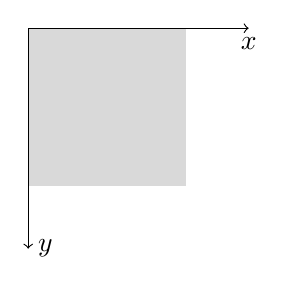
\begin{tikzpicture}[scale=1]
			\fill[fill=black!15!white] (0,0) rectangle (2,-2);
			\draw[->] (0,0) -- (0,-2.8) node[right]{$y$};
			\draw[->] (0,0) -- (2.8,0) node[below]{$x$};
		\end{tikzpicture}
		\caption{A \texttt{<div>} element.}
		\label{fig:sub2}
	\end{subfigure}
	\caption{Only a square crop-out of the original dartboard will be visible in this \texttt{<div>}.}
	\label{fig:test}
\end{figure}
\noindent In our case, the bulls-eye of the dartboard is located at around $20\%$ of the width and $60\%$ of the height of the picture respectively, with respect to the top left corner. The \texttt{HTML} might look something like
\begin{verbatim}
<div>
    <img src='dartboard.jpg' draggable='false' />
</div>
\end{verbatim}
\noindent and the accompanying \texttt{CSS}:
\begin{verbatim}
div {
    width: 500px;
    height: 500px;
    position: relative; /* so <img> can have absolute position */
}

img {
    position: absolute;
    height: auto; /* preserve aspect ratio, based on width */
    width: ??;
    left: ??;
    top: ??;
}
\end{verbatim}
\noindent The \texttt{width}, \texttt{left} and \texttt{right} properties of the picture are what we want to know.

\section{Mathematical analysis}
\noindent The \texttt{<div>} uses relative coordinates, which means the origin is at its top left corner and the $y$-value increases downwards (as seen in the diagram). However, in this analysis we will draw our coordinate systems in the conventional way, so to visualize what's happening one must reflect the image on the website across a horizontal line.

\enter In the diagram below, $c$ and $d$ denote the prescribed width and height of the area respectively, and the point $(a,b)$ the desired placement of the point of focus of the picture within this area. In the implementation it is key that these values are concrete \texttt{CSS} units, like \texttt{px} or \texttt{vw}.

\begin{figure}[H]
	\centering
	\begin{minipage}{.35\textwidth}
		\centering
		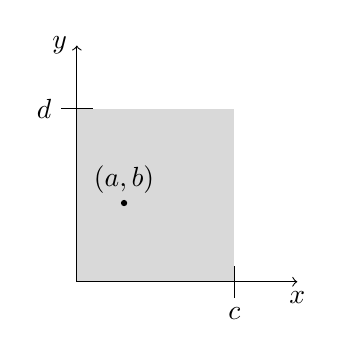
\begin{tikzpicture}[scale=1]
			\fill[fill=black!15!white] (0,0) rectangle (2,2.2);
			\draw[->] (0,0) -- (0,3) node[left]{$y$};
			\draw[->] (0,0) -- (2.8,0) node[below]{$x$};
			\draw (2,0.2) -- (2,-0.2) node[below] {$c$};
			\draw (0.2,2.2) -- (-0.2,2.2) node[left] {$d$};
			\fill (0.6,1) circle (0.04) node[above] {$(a,b)$};
		\end{tikzpicture}
		\captionof{figure}{Mathematical model of the \texttt{<div>} element.}
	\end{minipage}
	\hfill
	\begin{minipage}{.60\textwidth}
		\centering
		\begin{tikzpicture}[scale=1]
			\begin{scope}[shift={(-2.5cm,0.5cm)}]
				\begin{scope}[xshift=-2cm]
					\draw (0,0) rectangle (1cm,1cm);
					\fill (0.167cm,0.35cm) circle (0.04cm) node[anchor=south west,xshift=-0.1cm]{\small $(x,y)$};
					\draw[->] (1.2cm,0.5cm) -- (1.8cm,0.5cm);
				\end{scope}
			
			\draw[color=black!20!white] (0,0) rectangle (1.5cm,1cm);
			\draw[->] (0,0) -- (1.5cm,1cm) node[anchor=south west] {$r$};
			\fill (0.25cm,0.35cm) circle (0.04cm) node[anchor=south]{\small $z$};
			\draw[->] (1.7cm,0.5cm) -- node[pos=0.5,below]{$\lambda$} (2.3cm,0.5cm);
			\end{scope}
			
			\node[inner sep=0pt, opacity=.3] at (1.5cm,1cm)		{\includegraphics[height=2cm]{../dartboard.jpg}};
			%\draw[->] (0,0) -- (3.5cm,0);
			%\draw[->] (0,0) -- (0,2.5cm);
			\draw[] (0,0) -- (0.5cm,0.7cm);
			\draw[->] (0,0)  --(3cm,2cm) node[anchor=south west]{$\lambda r$};
			\fill (0.5cm,0.7cm) circle (0.06cm) node[above] {$\lambda z$};
			
		\end{tikzpicture}
		\captionof{figure}{Getting the focus vector and rescaling the picture with the ratio vector.}
	\end{minipage}
\end{figure}

\enter We will represent the \df{focus point} of the image by a pair of numbers $(x,y)\in [0,1]^2$, both between $0$ and $1$. So a value like $(0.2,0.6)$ would correspond to a focus point that is $20\%$ horizontally and $60\%$ vertically from the top left corner of an image.

\enter Let $w$ and $h$ respectively denote the width and height of the image, and let $R=w/h$ be the aspect ratio. Then we will denote by $r$ the \df{ratio vector} $(R,1)$. We may additionally think of the set $M=[0,R]\times [0,1]$ as a kind of idealized or unit picture, in that the set $\lambda M$ will always have the same aspect ratio as the picture, no matter which scaling factor $\lambda$ we pick. Notice that $(x,y)\mapsto (R\cdot x,y)$ is a bijection between $[0,1]^2$ and $M$, so the the focus point $(x,y)$ corresponds to the \df{focus vector} $z=(R\cdot x,y)$.

\enter Now, consider the two rays $\gamma,\delta$ starting from $(a,b)$, given by $\gamma(t)=(a,b)+t(r-z)$ and $\delta(t)=(a,b)-tz$. The vector $r-z$ can be found as the arrow pointing from $z$ to $r$. And we have $\gamma(t)-\delta(t)=tr$, so at any $t$ the points $\gamma(t)$ and $\delta(t)$ are the corners of the image scaled by a certain factor.
\begin{figure}[H]
	\centering
	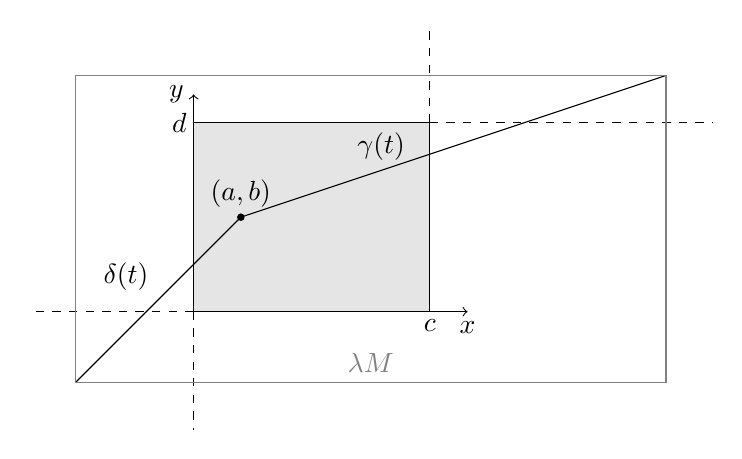
\begin{tikzpicture}[scale=0.6]
		\filldraw[fill=black!10!white] (0,0) rectangle (5,4);
		\draw[->] (0,0) -- (5.8,0) node[below]{$x$};
		\draw[->] (0,0) -- (0,4.6) node[left]{$y$};
		\node at (5,-0.3) {$c$};
		\node at (-0.3,4) {$d$};
		\draw[dashed] (5,4) -- (5,6);
		\draw[dashed] (5,4) -- (11,4);
		\draw[dashed] (0,0) -- (-3.5,0);
		\draw[dashed] (0,0) -- (0,-2.5);
		\draw (-2.5,-1.5) -- node[pos=0.5,anchor=south east]{$\delta(t)$} (1,2) -- node[pos=0.33,above]{$\gamma(t)$} (10,5);
		\fill (1,2) circle (0.08) node[above]{$(a,b)$};
		\draw[black!50!white] (-2.5,-1.5) -- (-2.5,5) -- (10,5) -- (10,-1.5) -- node[pos=0.5,above]{$\lambda M$} (-2.5,-1.5);
	\end{tikzpicture}
\end{figure}
\noindent Note that $r-z=(R,1)-(Rx,y)=(R(1-x),1-y)$. In order for the image determined by these endpoints to cover the area, we must have
\[
	\begin{aligned}[rl]
		\gamma_1(t) = a+tR(1-x) &\geq c \\
		\gamma_2(t) = b+t(1-y) &\geq d \\
		\delta_1(t) = a-tRx & \leq 0 \\
		\delta_2(t) = b-ty & \leq 0
	\end{aligned} \quad \iff \quad \begin{aligned}[rl]
		t & \geq \frac{c-a}{R(1-x)} \\
		t & \geq \frac{d-b}{1-y} \\
		t & \geq \frac{a}{Rx} \\
		t & \geq \frac{b}{y}.
\end{aligned}
\]
So make sure all of these conditions are satisfied simultaneously, we will take as our scaling factor
\[
	\lambda=\max \left\{ \frac{c-a}{R(1-x)} , \frac{d-b}{1-y} , \frac{a}{Rx}, \frac{b}{y} \right\}.
\]
Then $\texttt{width}=\pi_1(\lambda r)=\lambda R$, $\texttt{left} = \delta_1(\lambda)=a-\lambda Rx$ and $\texttt{top} = \delta_2(\lambda)=b-\lambda y$.


\end{document}
